\documentclass[a4paper,10pt]{article}
% - a4paper: printing paper format
% - 10pt: size of the characters

\usepackage{graphicx}
\usepackage{titling}
\usepackage{listings}
\usepackage[table]{xcolor}
\newcolumntype{R}[1]{>{\raggedleft\arraybackslash }b{#1}}
\newcolumntype{L}[1]{>{\raggedright\arraybackslash }b{#1}}
\newcolumntype{C}[1]{>{\centering\arraybackslash }b{#1}}
\lstset{%
  basicstyle=\scriptsize\sffamily,%
  commentstyle=\footnotesize\ttfamily,%
  frameround=trBL,
  frame=single,
  breaklines=true,
  showstringspaces=false,
  numbers=left,
  numberstyle=\tiny,
  numbersep=10pt,
  keywordstyle=\bf
}
\newcommand{\subtitle}[1]{%
  \posttitle{%
    \par\end{center}
    \begin{center}\large#1\end{center}
    \vskip0.5em}%
}



%%%%%%%%%%%%%%%%%%%%%%%%%%%%%%%%%%%%%%%%%%%%%%%%%%%%
%				Title / Subtitle / Authors and Date									   %
% This should be adapted to your report.					                                                              %
%																			   %
%%%%%%%%%%%%%%%%%%%%%%%%%%%%%%%%%%%%%%%%%%%%%%%%%%%%
\title{TD3 : Formatted I/O Library}
\subtitle{Master M1 MOSIG, Grenoble Universities}
\author{Lenka Kun\'{i}kov\'{a} \and Lina Marsso}
\date{26/10/2014}

\begin{document}
% Beginning serious stuff. 


\maketitle
% Actually prints title / subtitle / authors and dat into the document


%%%%%%%%%%%%%%%%%%%%%%%%%%%%%%%%%%%%%%%%%%%%%%%%%%%%
%								Abstract										   %
% Change the part below the abstract so that it corresponds to your report	                                     %
%																			   %
%%%%%%%%%%%%%%%%%%%%%%%%%%%%%%%%%%%%%%%%%%%%%%%%%%%%

%%%%%%%%%%%%%%%%%%%%%%%%%%%%%%%%%%%%%%%%%%%%%%%%%%%%
%								Introductio	n									   %
%																			   %
% the command \section{name of the section} begins a new section of the document                            %
%																			   %
%%%%%%%%%%%%%%%%%%%%%%%%%%%%%%%%%%%%%%%%%%%%%%%%%%%%
\section{Introduction}
	\paragraph{}
	In this project we focus on input in and output from file. Our goal was to implement library usable for formatted I/O on top of the system calls read and write. In other words we try to reimplement few functions from standard library stdio.h, trying to reduce number of system calls needed using the buffer.
	\paragraph{}
	In the first part, we talk about few implementation details of our functions, later we show that we succeeded in our attempt to reduce number of system calls and illustrate how time costly this low level calls can be when we compare speed of two programs: one using only system calls and one using our small library my\_stdio.h.



\section{Implementation}	
\subsection{Struct my\_file}
 Our structure my\_file consists of buffer in which we temporarily store information that we read from a file or that user tried to write in. We use two pointers that show us in which part of the buffer are valid data. Of course, we need to remember handler we got from the system call write / read. We also have variables to distinguish between read and write mode, to remember if we already met EOF and one that knows whether buffer was already filled or it is empty.  
 \subsection{My\_fopen}
 In this function we allocate the memory needed for the whole structure and we initialise all variables. Both pointers will point to the beginning of the buffer. According to the specified mode we open the file with appropriate flags.
 \subsection{My\_fclose}
 In this function we need to close the file and free all allocated memory. If the mode of file is set to write, we also need to write the content of the buffer into the file.

 \subsection{My\_fread}
 At first, the function should check whether the mode is set to read, if not, it returns -1. Then we need to distinguish between different cases. In case it is the first read operation, the buffer is empty and we need to fill it. In case the amount of data the user requests to read is less than data available, it is the simplest case and we just give requested data to the user. Another case is when we meet EOF before expected. It can be detected thanks to the pointer that points to the end of valid data. In this case we just give user less data than he wanted. It can also happen that user wants more than what is disponsible in the buffer. In this case, we give him all we have, we refill the buffer and give him remaining data. We keep refilling data until we get enough.

 \subsection{My\_fwrite}
 As in the previous function, we should test whether the mode is set to write. If it is, user data will be stored. If there is enough space in the buffer, we just write all user data in. Once the buffer is full, we write its content in a file using actual system call. We keep writing data in and flushing full buffer until all user data are processed.

\subsection{My\_feof}
This function should say whether we met EOF during previous read. For this purpose we use variable defined in struct my\_file, which is updated in function my\_fread when EOF is recognized. Here we just return its value.

\subsection{My\_fprintf}
During implementation of this function we needed to deal with list of arguments of variable length. To work with them we use variable of type va\_list. The function processes string format in a while cycle. All normal characters are directly written using my\_fwrite function. When we reach character '\%', we switch to one of three possibilities(\%d, \%s, \%c). When we are dealing with one character (\%c), we pop the argument from va\_list, and we write its value to the file. When we are dealing with whole string, first we need to discover the length of it using strlen. Then we write appropriate number of characters stored in argument to the file. When we reach \%d we need to transform integer value to a char, then we can write it. While cycle ends when we reach \textbackslash 0 and during whole cycle we count number of successfully processed arguments.
\subsection{My\_fscanf}
Function is very similar to previous one but it is a bit more complicated. In case of \%s, for example, we do not know the length of string at the beginning. We read characters from file one by one and we look for white characters. When we reach one, we assume it is the end of string. We add \textbackslash 0 to the end and we give it back to user. For \%d it is similar. We recognize end of the number when we read first non-digit character.
\section{Evaluation}
\paragraph{}
To evaluate our library, we used the test that copies one file to an other file using our library (buffered write and read) and did the same  using the standard system calls open, read and write.
\paragraph{}
We evaluated at the beginning the time required for coping two files with our library,  
and with the standard system calls open, read and write. We have also one ratio~: 
\begin{equation}
\left(\frac{My\_stdio\_time\_execution}{Standar\_Read\_Write\_time\_execution} \right)  \quad
\end{equation}
\paragraph{}
We calculated the time of the execution with a script time.sh. We can see

\begin{tabular}{|R{2cm}|C{2cm}|L{1.5cm}|L{1.5cm}|}
\hline \rowcolor{lightgray}Library & Time (microsecondes) & Size of file\\
\hline  libmy\_sdio & 4 & 8.0K \\
\hline  Standar  & 36 & 8.0K \\
\hline 
\end{tabular}

\begin{figure}[ht]
\center 
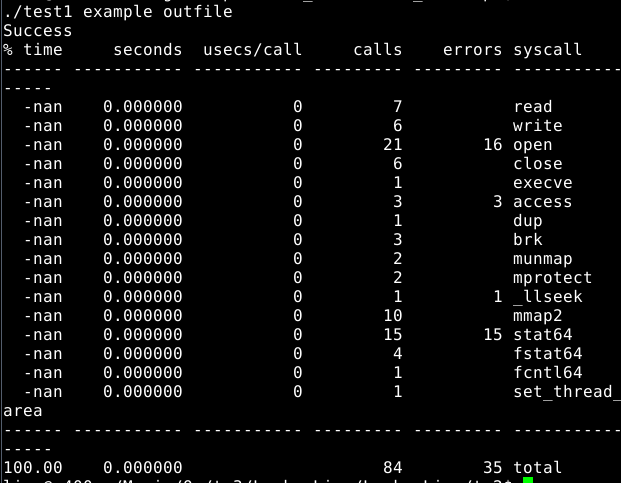
\includegraphics[width=0.85\linewidth]{my_strace.png}
\caption{Number of system call of our library}
\label{first}
\end{figure}
\begin{figure}[ht]
\center 
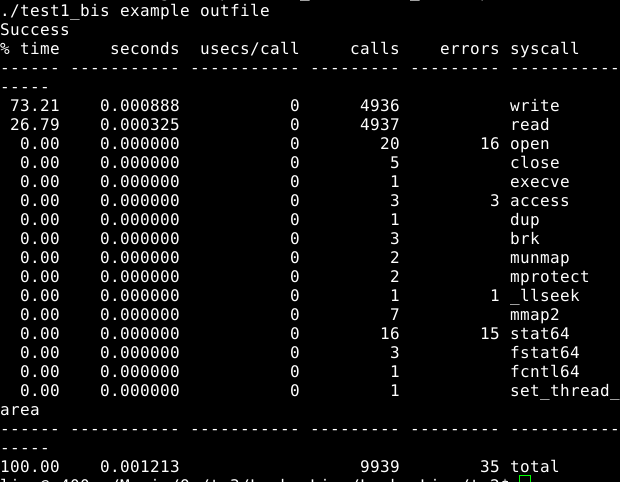
\includegraphics[width=0.85\linewidth]{syscall_strace.png}
\caption{Number of system call with read and write}
\label{worst}
\end{figure}
\begin{figure}[ht]
\center 
%\includegraphics[width=0.8\linewidth]{gcc_best_fit.png}

\label{best}
\end{figure}

\newpage


\section{Conclusion}
\paragraph{}
In this project we implemented library that provided high level interface to same basic input-output operations. We tested its behavior and compared program using it and program using only low level system calls. We showed that our library reduces the number of needed system calls, which largely affects the speed of the program. Both static and dynamic version of our library were created. 
\paragraph{} 
This task required a lot of effort and was very difficult for us to finish, as long as both of us are suffering illness since the beggining of the previous week. We both are excused from the doctor, we sent an e-mail regarding possible postponing of submitting this task and the second task, that we needed to deliver. As long as we did not receive an answer, we tried to do our best that our situation allowed us. The report may not be therefore perfect, but we hope our situation will be taken into account and hope for your understanding.

 \end{document}
